\documentclass{beamer}

\mode<presentation>{\usetheme{Madrid}}
\usepackage{graphicx}
\usepackage{multimedia}
\usepackage{hyperref}

\usepackage[utf8]{inputenc}
\usepackage[ngerman]{babel}
\usepackage{amsmath, amssymb, amsthm}

\usepackage{subcaption}
\usepackage[T1]{fontenc}
%\usepackage[sort&compress]{natbib}

\usepackage{lmodern}
\usepackage{caption}


\author[Jan Niclas Ruppenthal, Michael Feldmann, Philipp Geier]{}
\title[]{2. Übung zur Vorlesung
Virtual Reality\\ Circles of Life}
\institute[Universität Trier]{}
\date[06. Mai 2024]{}
\beamertemplatenavigationsymbolsempty
\setbeamertemplate{footline}
{
  \leavevmode%
  \hbox{%
  \begin{beamercolorbox}[wd=.50\paperwidth,ht=2.25ex,dp=1ex,center]{author in head/foot}%
    \usebeamerfont{author in head/foot}\insertshortauthor%~~\beamer@ifempty{\insertshortinstitute}{}{(\insertshortinstitute)}
  \end{beamercolorbox}%
  \begin{beamercolorbox}[wd=.50\paperwidth,ht=2.25ex,dp=1ex,right]{date in head/foot}%
    \usebeamerfont{date in head/foot}\insertshortdate{}\hspace*{2em}
    \insertframenumber{} / \inserttotalframenumber\hspace*{2ex} 
  \end{beamercolorbox}}%
  \vskip0pt%
}
%—-------------------------------------------------------------

\begin{document}
{
  \usebackgroundtemplate{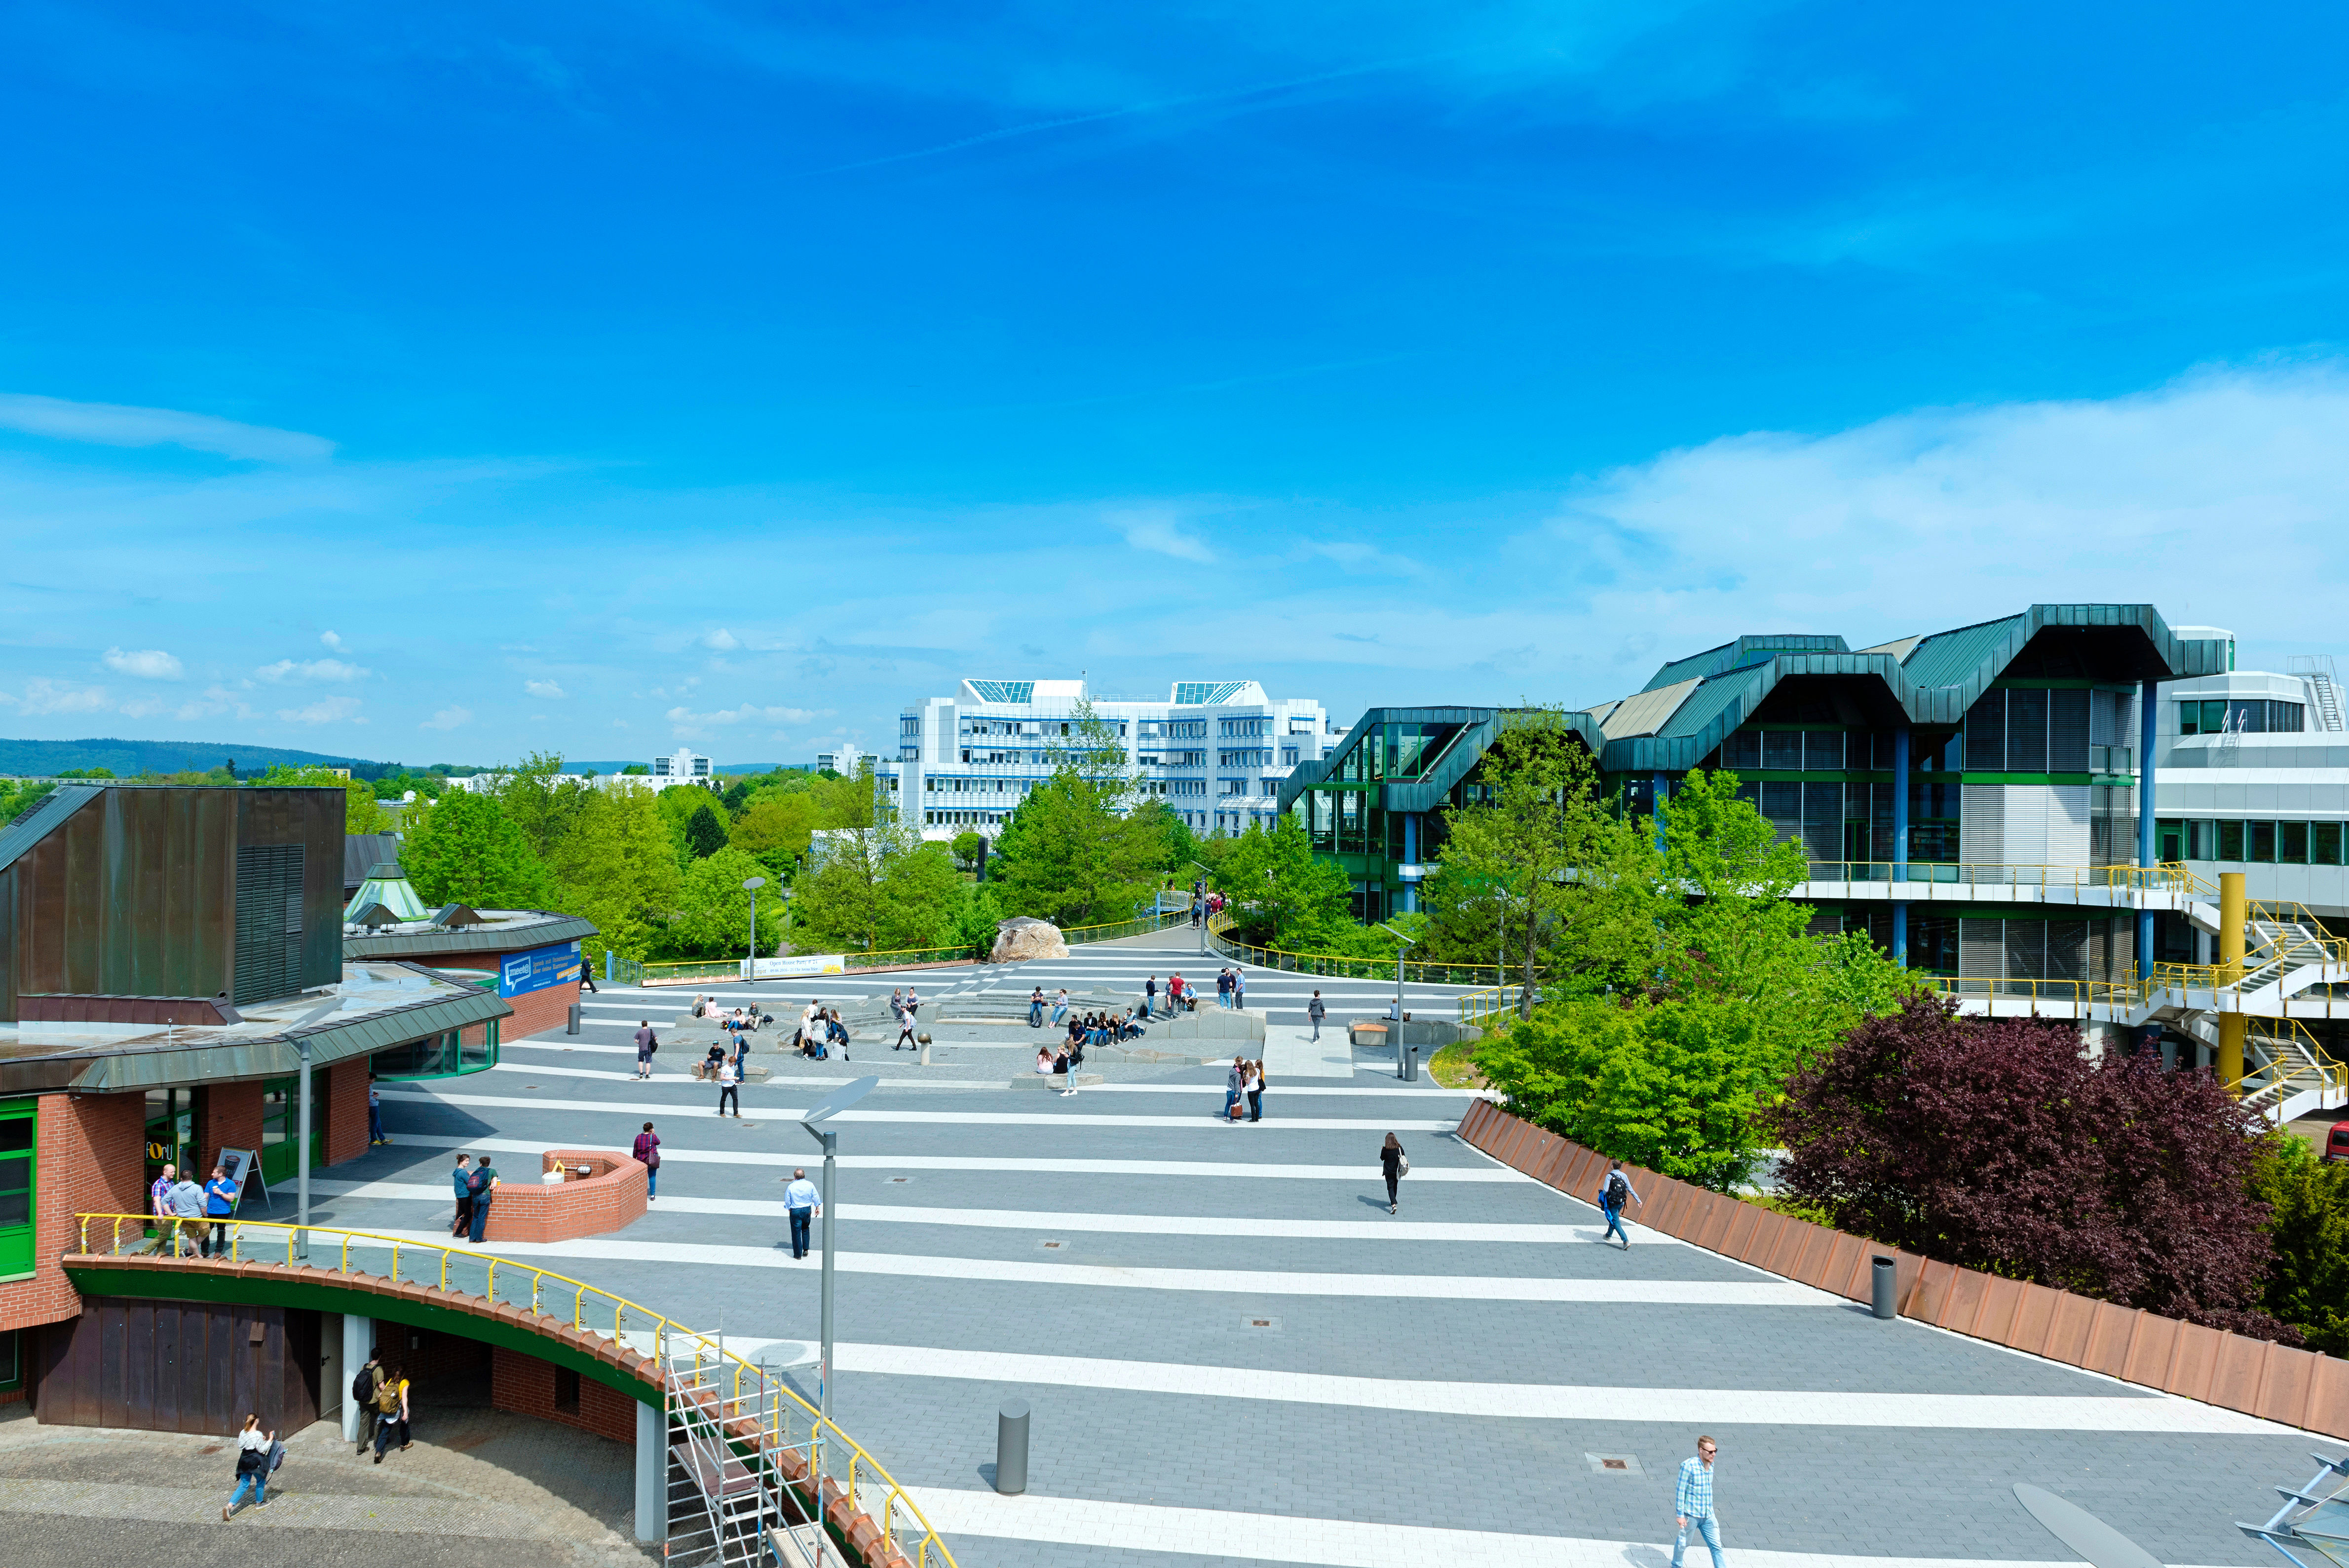
\includegraphics[width=1.2\paperwidth]{img/unitrier}}
  \begin{frame}
    \maketitle
  \end{frame}
}
    
    %\begin{frame}
       % \frametitle{Inhalt}
		%\tableofcontents
	%\end{frame}
	
%—------------------------------------------------------


\begin{frame}{Aufgabenteil A}
\begin{itemize}
\item Rotiere Baum entlang Stamm mit Geschwindigkeit 90°/s:
\end{itemize}
\begin{figure}
    \centering
    \movie[externalviewer]{
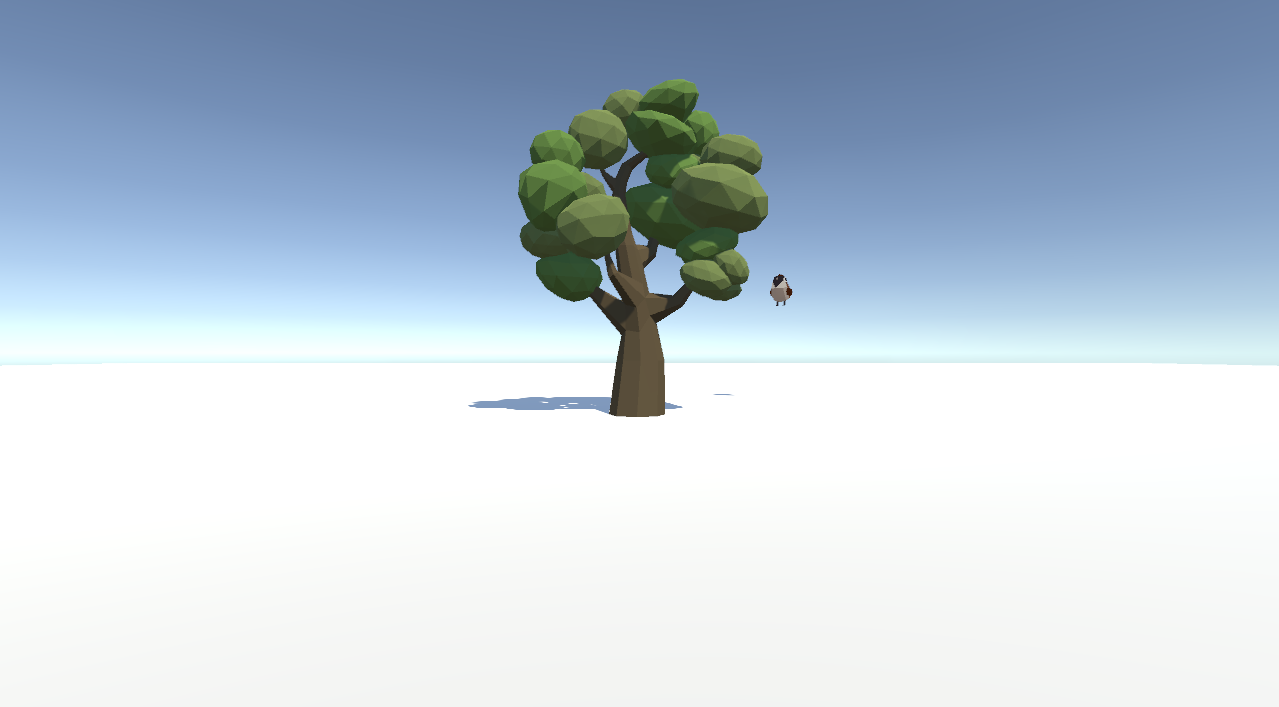
\includegraphics[width=0.9\textwidth, keepaspectratio]{img/aufgabeA}
}{vid/aufgabeA.mkv}
\end{figure}
\end{frame}

\begin{frame}{Aufgabenteil B}
\begin{itemize}
\item Geschwindigkeit variable zwischen -180°/s und 180°/s:
\end{itemize}
\begin{figure}
    \centering
    \movie[externalviewer]{
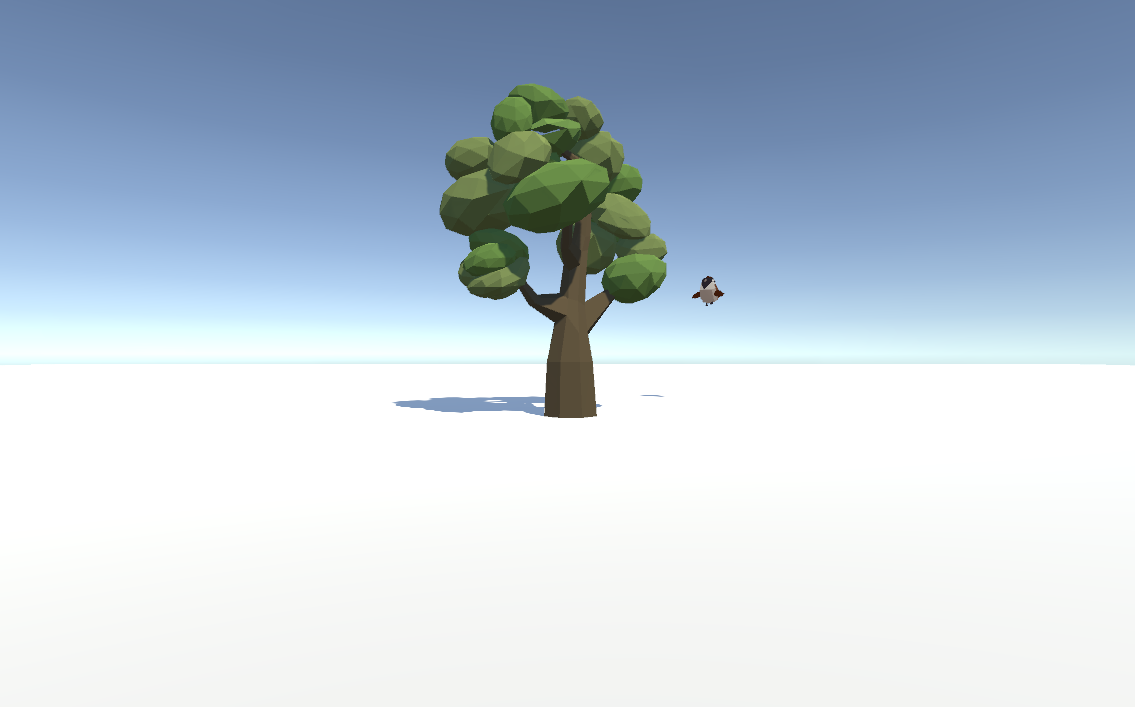
\includegraphics[width=0.9\textwidth, keepaspectratio]{img/aufgabeB}
}{vid/aufgabeB.mkv}
\end{figure}
\end{frame}

\begin{frame}{Aufgabenteil C}
\begin{itemize}
\item Spatz und Baum drehen sich:
\end{itemize}
\begin{figure}
    \centering
    \movie[externalviewer]{
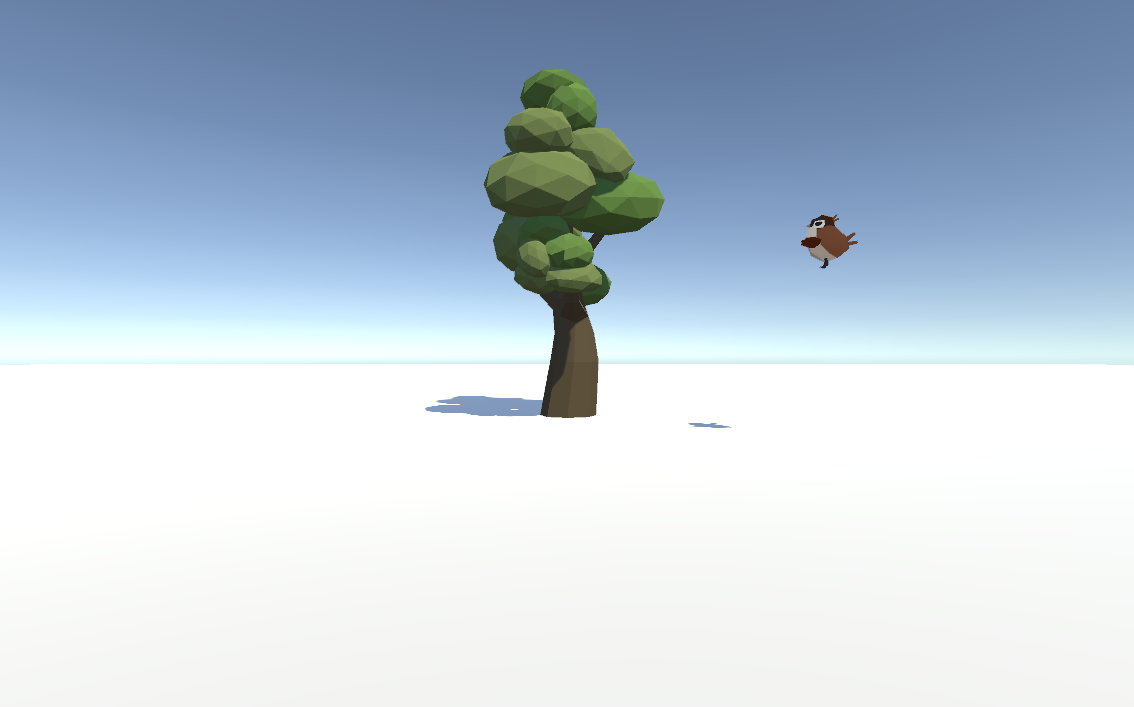
\includegraphics[width=0.9\textwidth, keepaspectratio]{img/aufgabeC}
}{vid/aufgabeC.mkv}
\end{figure}
\end{frame}

\begin{frame}{Aufgabenteil D}
\begin{itemize}
\item Nur der Spatz dreht sich:
\end{itemize}
\begin{figure}
    \centering
    \movie[externalviewer]{
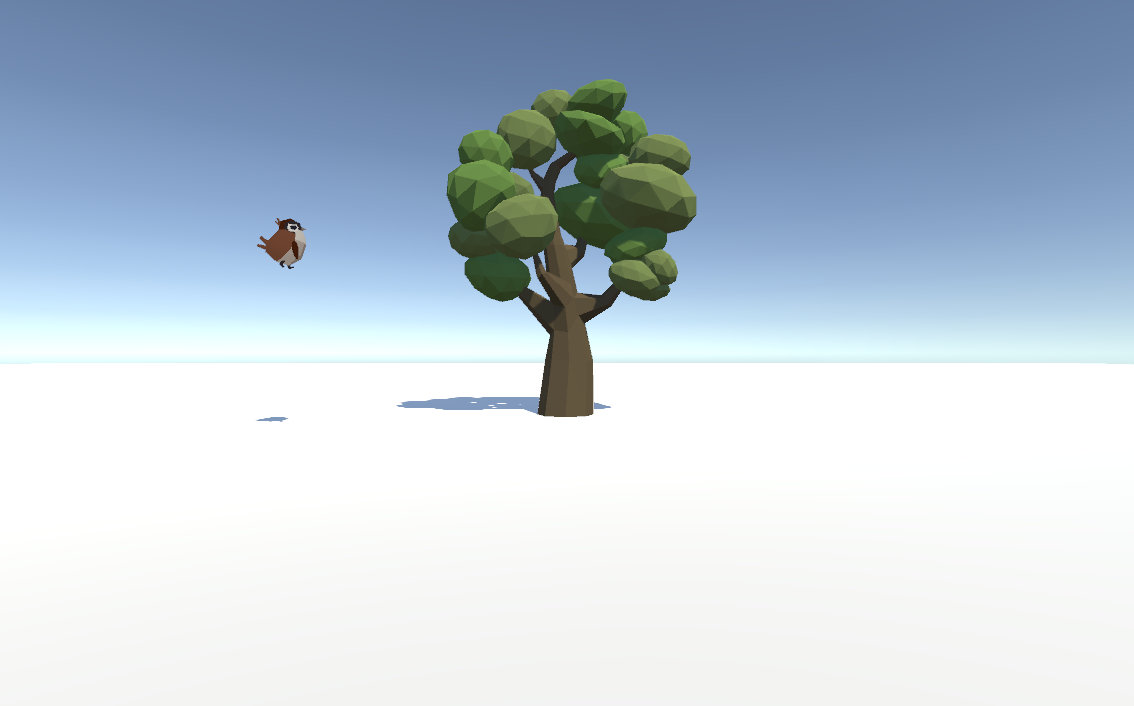
\includegraphics[width=0.9\textwidth, keepaspectratio]{img/aufgabeD}
}{vid/aufgabeD.mkv}
\end{figure}
\end{frame}

\begin{frame}{Aufgabenteil E}
\begin{itemize}
\item Spatz fliegt um den Baum und schaut nach vorne:
\end{itemize}
\begin{figure}
    \centering
    \movie[externalviewer]{
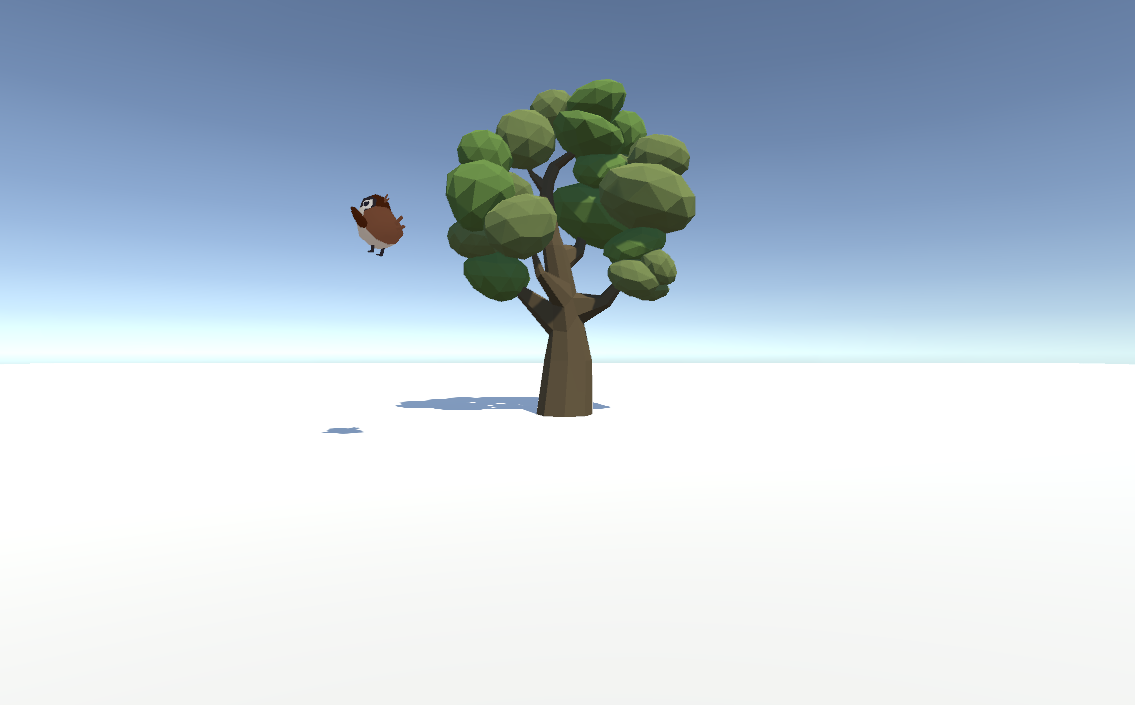
\includegraphics[width=0.9\textwidth, keepaspectratio]{img/aufgabeE}
}{vid/aufgabeE.mkv}
\end{figure}
\end{frame}

\begin{frame}{Aufgabenteil F}
\begin{itemize}
\item Bäume wachsen und zerfallen, der Spatz sucht sich den größten:
\end{itemize}
\begin{figure}
    \centering
    \movie[externalviewer]{
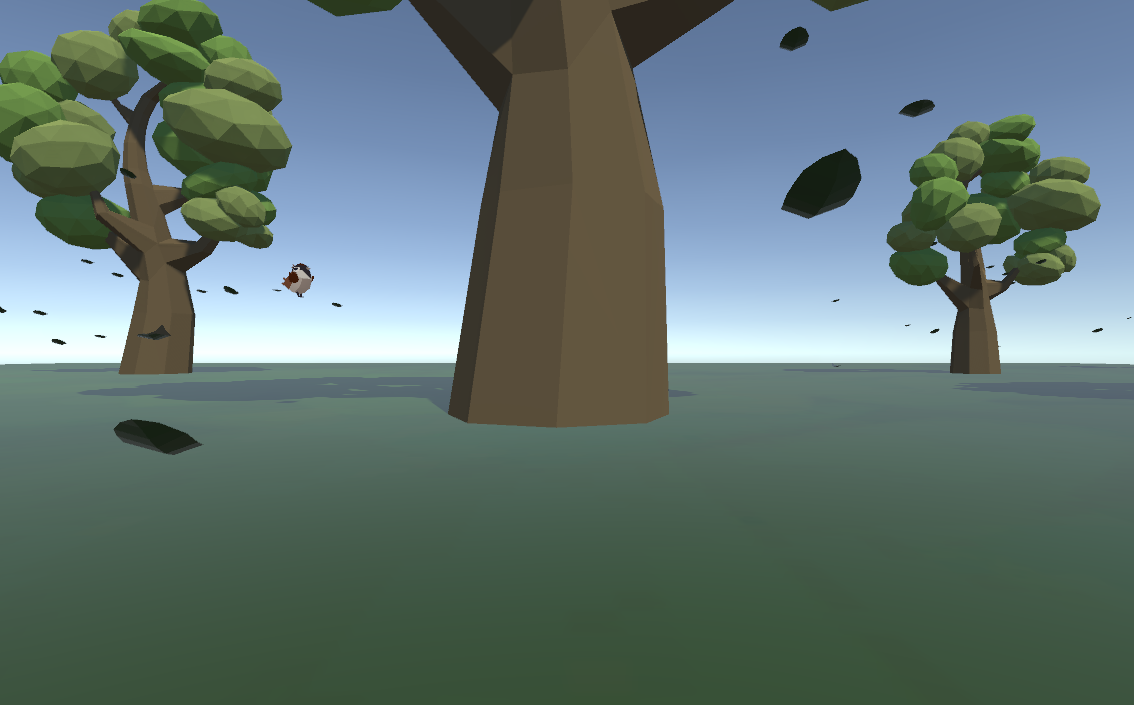
\includegraphics[width=0.9\textwidth, keepaspectratio]{img/aufgabeF}
}{vid/aufgabeF.mkv}
\end{figure}
\end{frame}

\begin{frame}{Aufgabenteil G}
\begin{itemize}
\item Perspektivenwechsel:
\end{itemize}
\begin{figure}
    \centering
    \movie[externalviewer]{
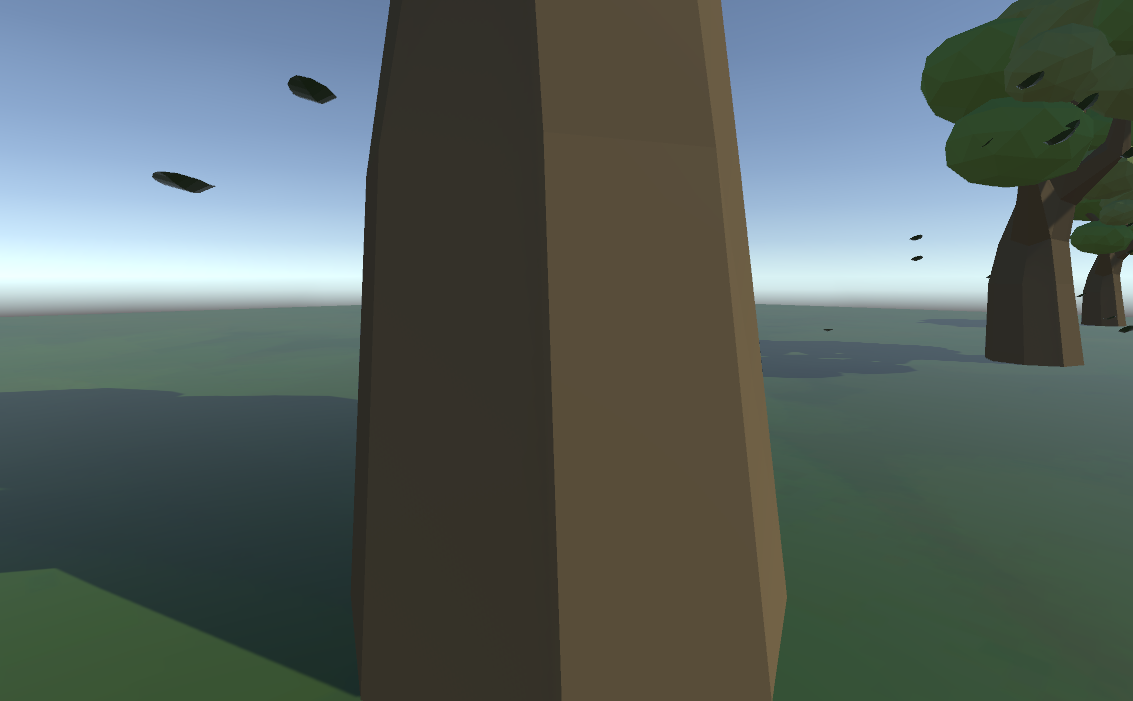
\includegraphics[width=0.9\textwidth, keepaspectratio]{img/aufgabeG}
}{vid/aufgabeG.mkv}
\end{figure}
\end{frame}

\begin{frame}{Brainstorming}
\begin{itemize}
\item Was können wir mit einem sich bewegenden Vogel machen?
\item Wie können wir den Nutzer mit einbringen?
\item Wie könnte eine Gamification aussehen?
\end{itemize}
\end{frame}

\begin{frame}{Aufgabenteil H}
\begin{itemize}
\item ANGRY BIRDS!!!
\end{itemize}
\begin{figure}
    \centering
    \movie[externalviewer]{
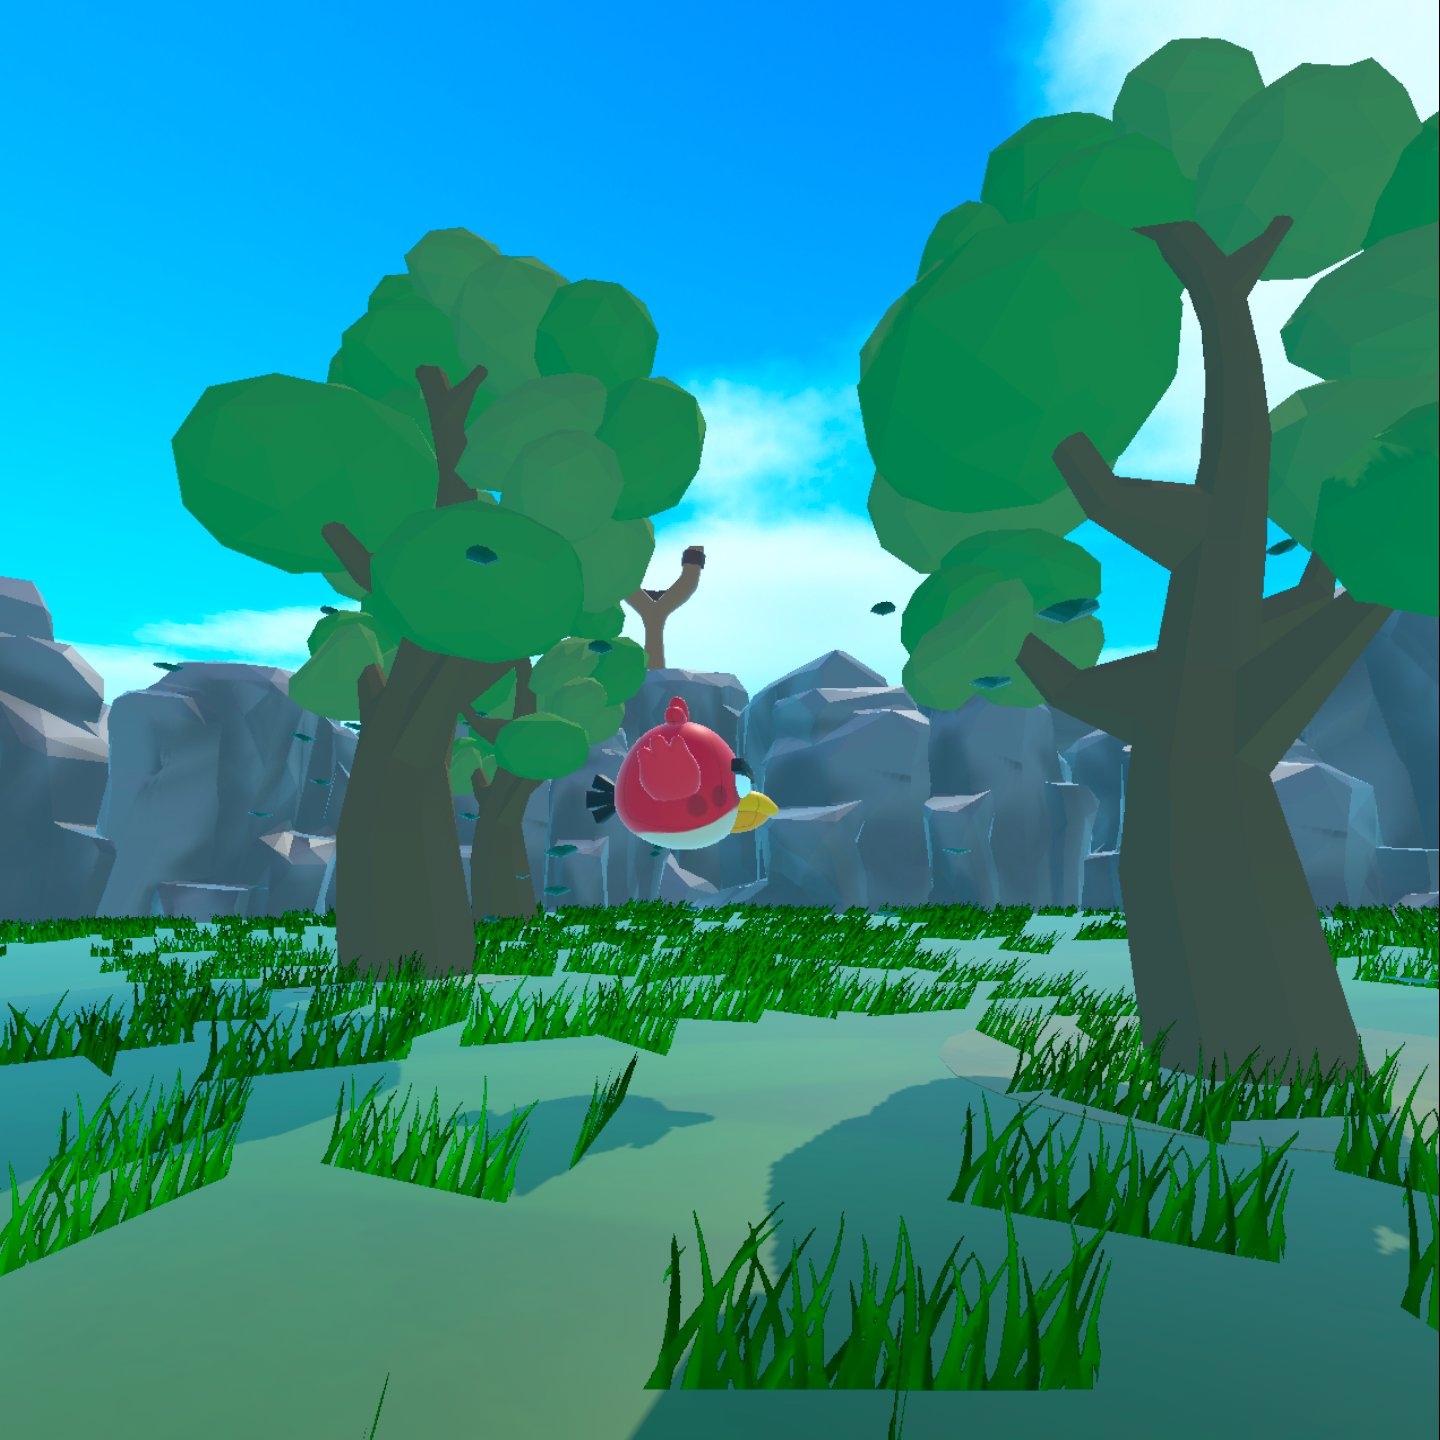
\includegraphics[height=0.8\textheight, keepaspectratio]{img/aufgabeH}
}{vid/aufgabeH.mp4}
\end{figure}
\end{frame}



\begin{frame}{Quellen}
	\begin{thebibliography}{1}
\bibitem{nick}[1]{ siehe README.txt}
\end{thebibliography}
\end{frame}


	
    	
    	
    	
\end{document}
